\documentclass[12pt,letterpaper]{article}
\usepackage[utf8]{inputenc}
\usepackage[spanish]{babel}
\usepackage{amsmath}
\usepackage{color}
\usepackage{algorithm}
\usepackage[noend]{algpseudocode}
\renewcommand{\algorithmicrequire}{\textbf{Entrada:}}
\renewcommand{\algorithmicensure}{\textbf{Salida:}}
\usepackage{subcaption}
\usepackage{amsfonts}
\usepackage{hyperref}
 \hypersetup{
     colorlinks=true,
     linkcolor=blue,
     filecolor=blue,
     citecolor = blue,      
     urlcolor=cyan,
     }
\usepackage{amssymb}
\usepackage{listings}

\usepackage{amsthm}
\newtheorem{theorem}{Teorema}

\usepackage{graphicx}
\usepackage[left=2cm,right=2cm,top=2cm,bottom=2cm]{geometry}
\setlength{\parskip}{3mm}
\title{\textsc{Distribución normal y uniforme}}
\author{\textsc{Fabiola Vázquez}}

\setlength{\parindent}{0cm}
\renewcommand{\lstlistingname}{Código}
\floatname{algorithm}{Algoritmo}
\begin{document}
\maketitle

\hrule
\section{Introducción}
En este estudio, que se realiza con el software estadístico R versión 4.0.2 \cite{R} en un cuaderno de Jupyter \cite{jupyter}, se trabaja con distintos algoritmos para la generación de valores con distrubución normal y uniforme.

\section{Generación de variables con distribución uniforme}
Uno de los métodos que existen para la generación de valores uniformemente distribuidos es el método congruencial, que sigue la siguiente relación $$x_{n+1}\equiv ax_n + c \mod m$$ Para este método necesitamos los parámetros enteros \texttt{a}, \texttt{c}, \texttt{m} y una \texttt{semilla}. 

Como un primer ejemplo, se considera un generador congruencial con \texttt{m}=8, \texttt{a}=5, \texttt{c}=4. Si en la función, que se muestra en el código \ref{lst:gc1}, se hace \texttt{semilla} = 5 y se pide \texttt{uniforme(10,5)}, el generador solo nos regresa el mismo valor diez veces, es decir, la elección de parámetros no es la indicada.

\begin{lstlisting}[label=lst:gc1,caption=Generador congruencial., frame = single]
uniforme = function(n, semilla) {
    a = 5
    c = 4
    m = 8
    
    datos = numeric()
    x = semilla
    
    while (length(datos)<n){
        x=(a*x + c) %%   m
        datos=c(datos,x)
    }
    return(datos/(m-1))
}
\end{lstlisting} 

Se debe garantizar que el ciclo del generador congruencial sea de ciclo máximo o muy grande. El siguiente teorema  muestra las propiedades que deben cumplir los parámetros para que se tenga periodo máximo \cite{int}.
\begin{theorem}
Las siguientes condiciones son necesarias y suficientes para que un generador congruencial con parámetros $m, a$ y $c$, tengan período máximo.
\begin{enumerate}
\item $c$ y $m$ son primos relativos (i.e. m.c.d. ($c$,$m$)=1).
\item $a-1$ es múltiplo de todos los factores primos de $m$ (i.e. $a\equiv 1 \mod g,$ para todo $g$ factor primo de $m$).
\item Si $m$ es múltiplo de cuatro, entonces $a-1$ también lo ha de ser (i.e. $m\equiv 0 \mod 4 \Rightarrow a \equiv 1 \mod 4$).
\end{enumerate}
\end{theorem}

Con lo anterior, es fácil ver que, si tenemos a \texttt{m} como una potencia de dos, basta con que \texttt{c} y \texttt{a} sean números impares, con esto se modifican los parámetros de la función \texttt{uniforme} y se tiene como en el código \ref{lst:gc2}, el cuál es un generador de ciclo máximo.
\begin{lstlisting}[label=lst:gc2,caption=Generador congruencial., frame = single]
uniforme = function(n, semilla) {
    a = 16385
    c = 8191
    m = 65536
    
    datos = numeric()
    x = semilla
    
    while (length(datos)<n){
        x=(a*x + c) %%   m
        datos=c(datos,x)
    }
    return(datos/(m-1))
}
\end{lstlisting} 

Se llama la librería \texttt{uniftest} y se utiliza la función \texttt{sherman.unif.test} para realizar un prueba de uniformidad de Sherman a una muestra de los números que se generan. La prueba arroja un \texttt{valor p} de 0.9925 y al ser mayor que 0.05, se acepta la hipótesis de que los números se distribuyen uniformemente.



\section{Generación de variables con distribución normal}
Se estudian tres diferentes algoritmos que generan valores con distribución normal.
\subsection{Algoritmo Box-Müller}
Este algoritmo, usa dos variables uniformemente distribuidas independientes para la generación de dos valores independientes con distribución normal \cite{int}. 

\begin{algorithm}
  \caption{Algoritmo Box-Müller}
  \begin{algorithmic}[1]
    \Require{$\mu, \sigma$} 
    \Ensure{$z_0, z_1$ variables con distribución normal}
 
    \State Generar  $u_1, u_2 \sim U(0,1)$ 
    \State Hacer $x_1=\sqrt{-2\ln(u_1)}\cos( 2\pi u_2)$ y $x_2=\sqrt{-2\ln(u_1)}\sen( 2\pi u_2)$
    \State Devolver $z_1=\mu + \sigma \cdot z_1$ y $z_2=\mu + \sigma \cdot z_2$
 
  \end{algorithmic}
\end{algorithm}

Se realizan tres experimentos distintos, uno con ambas variables que retorna el algoritmo, y otros dos eligiendo solo una de las dos. Se quiere ver si hay alguna diferencia significativa entre los experimentos. En cada uno de estos, se generan 500 replicas de 5000 , donde a cada una de las replicas se le realiza una prueba de normalidad de Shapiro y 469 obtuvieron un \texttt{valor p} mayo de 0.05. En la figura \ref{boxmuller} se tiene los histogramas de una de las 500 réplicas considerando las variaciones del algoritmo y se compara con los generados usando la función \texttt{rnorm}.



\begin{figure}
\centering
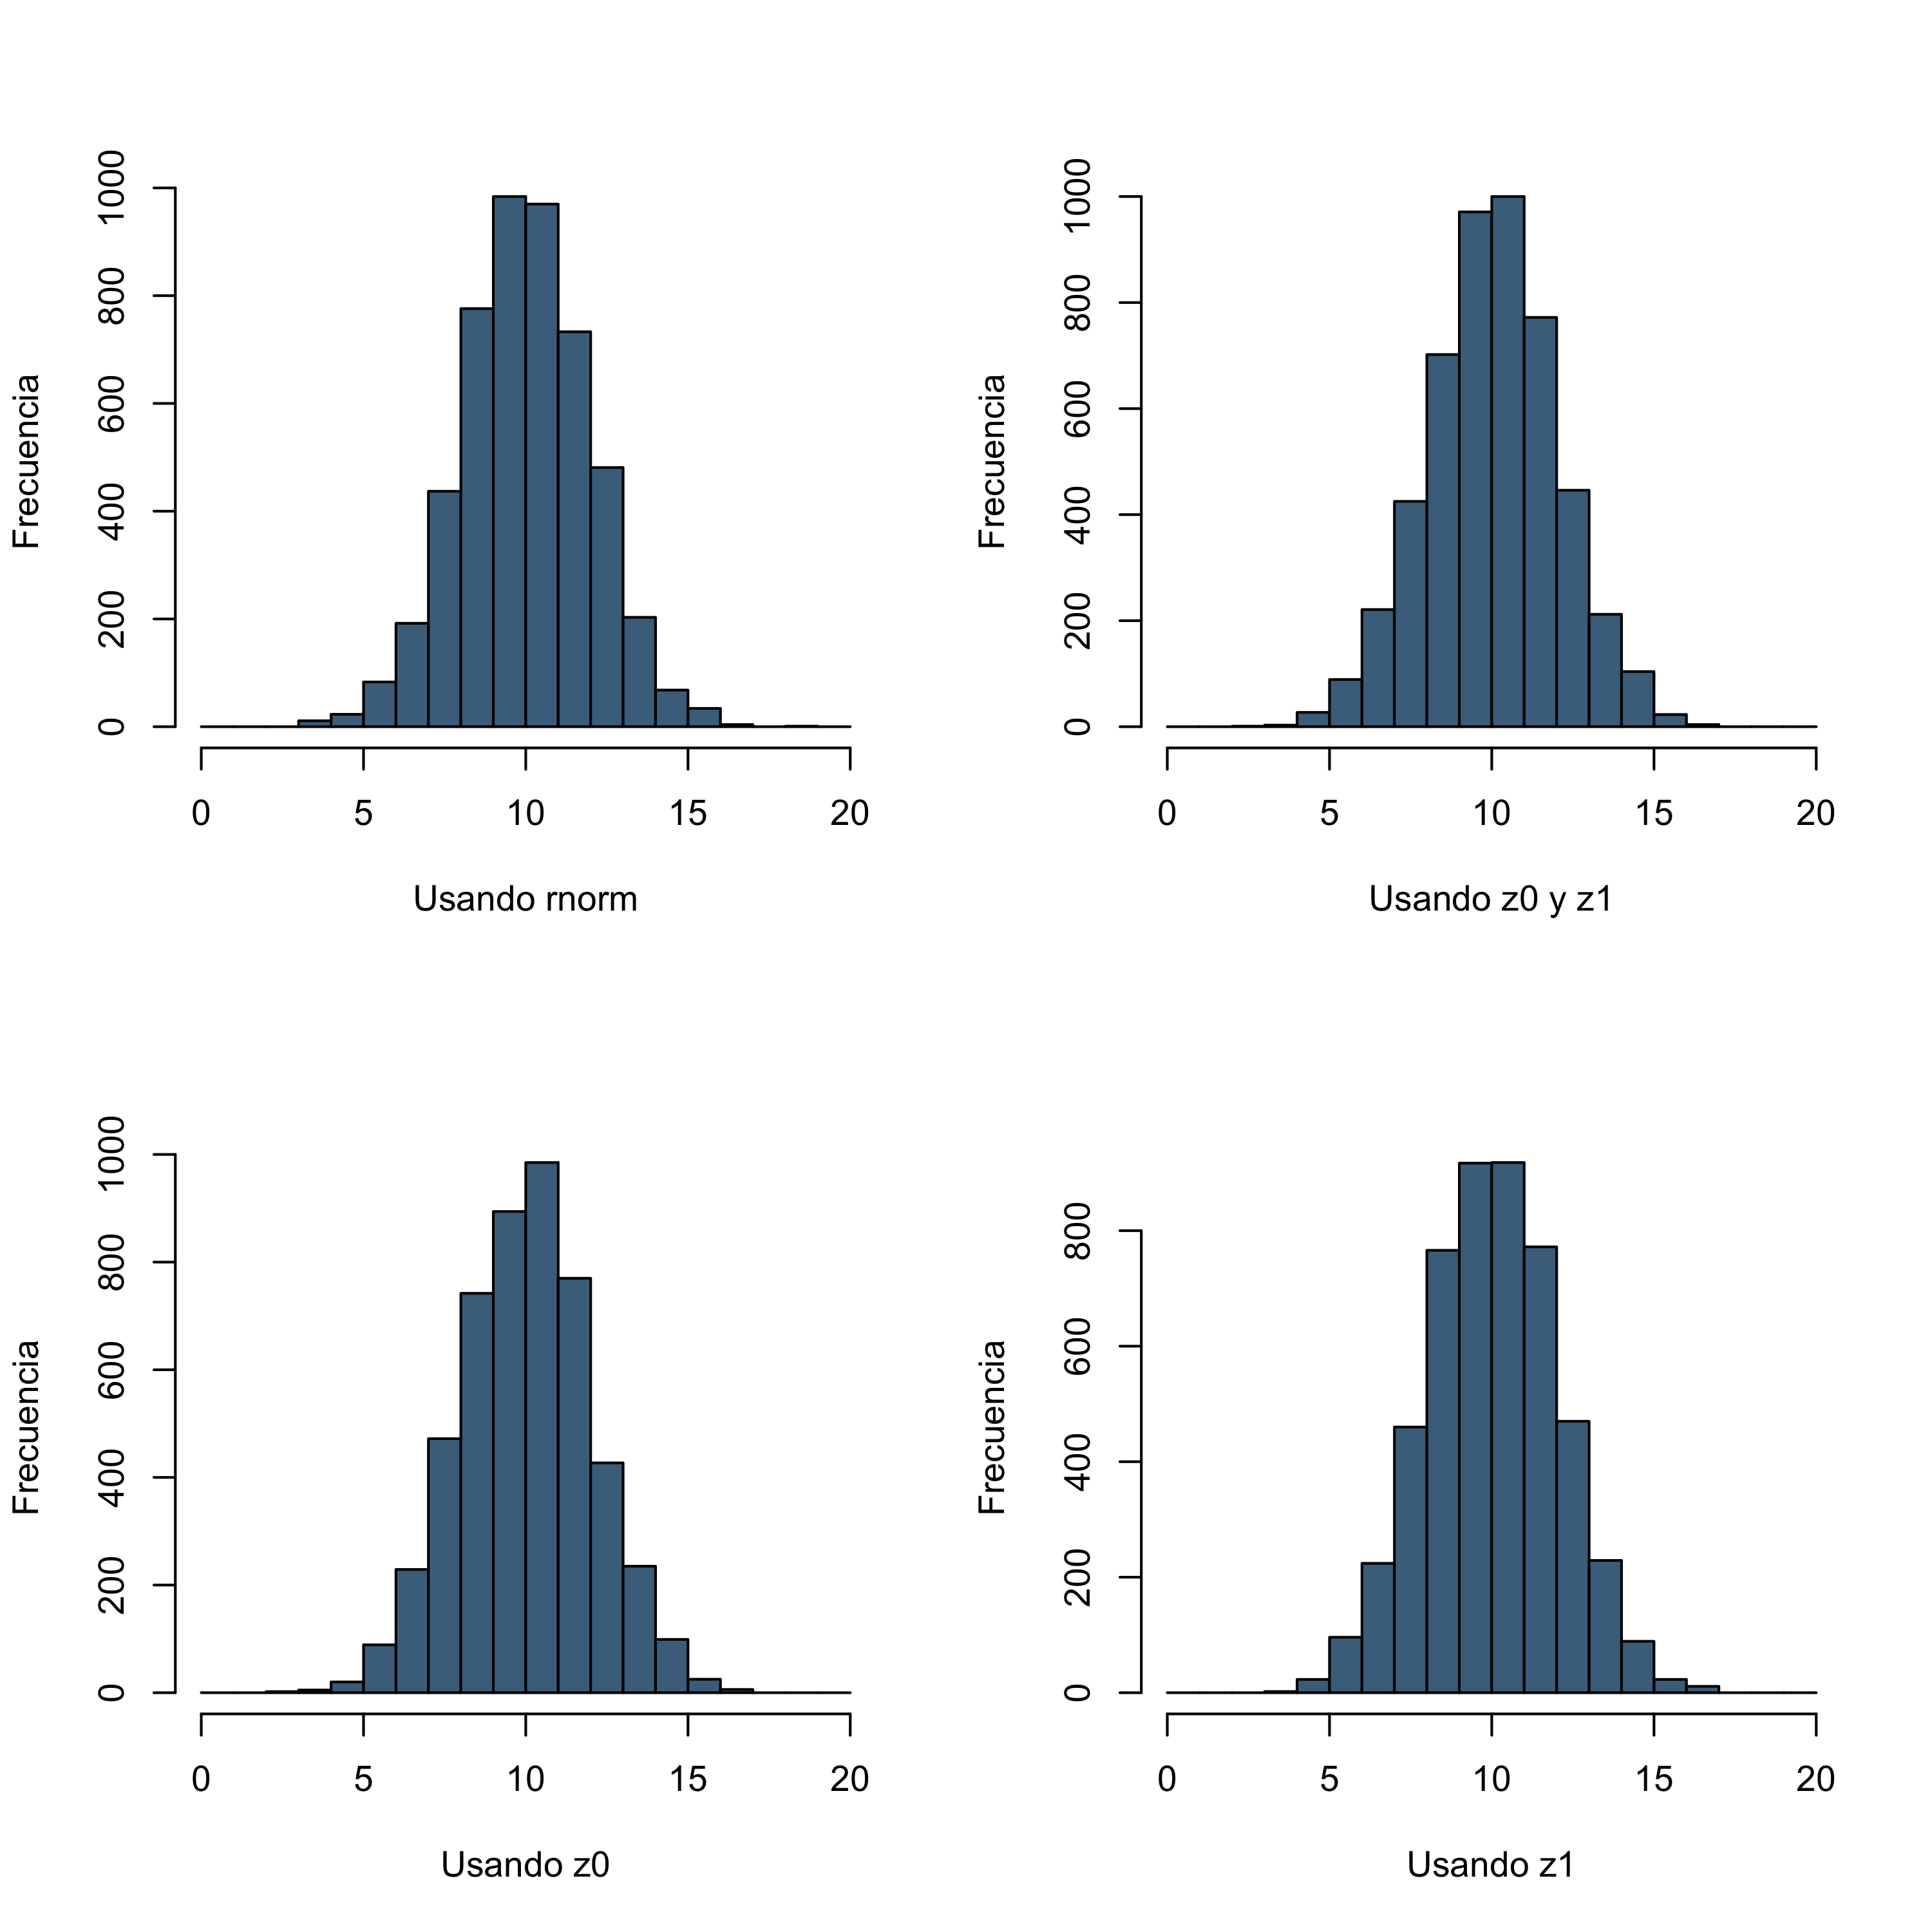
\includegraphics[scale=0.12]{boxmuller.png}
\caption{Histogramas de una réplica con las variaciones del algoritmo de Box-Muller.} 	
\label{boxmuller}
\end{figure} 


\subsection{Algoritmo polar}
Otro algoritmo para la generación de variables normalmente  distribuidas es el \textit{Algoritmo polar} \cite{int}. 

\begin{algorithm}
  \caption{Algoritmo polar}
  \begin{algorithmic}[1]
    \Ensure{$z_0, z_1$ variables con distribución normal}
 
    \State Generar  $u_1, u_2 \sim U(0,1)$ 
    \State Hacer $v_1 = 2u_1 - 1 $, $v_2=2u_2 - 1$ y $w=v_1^2 + v_2^2$
    \State Si $w>1$ entonces, volver a 1
    \State Hacer $y=\sqrt{\frac{-2\ln w}{w}}$
    \State Devolver $x_1=v_1 y$, $x_2=v_2 y$
 
  \end{algorithmic}
\end{algorithm}

\begin{figure}
\centering
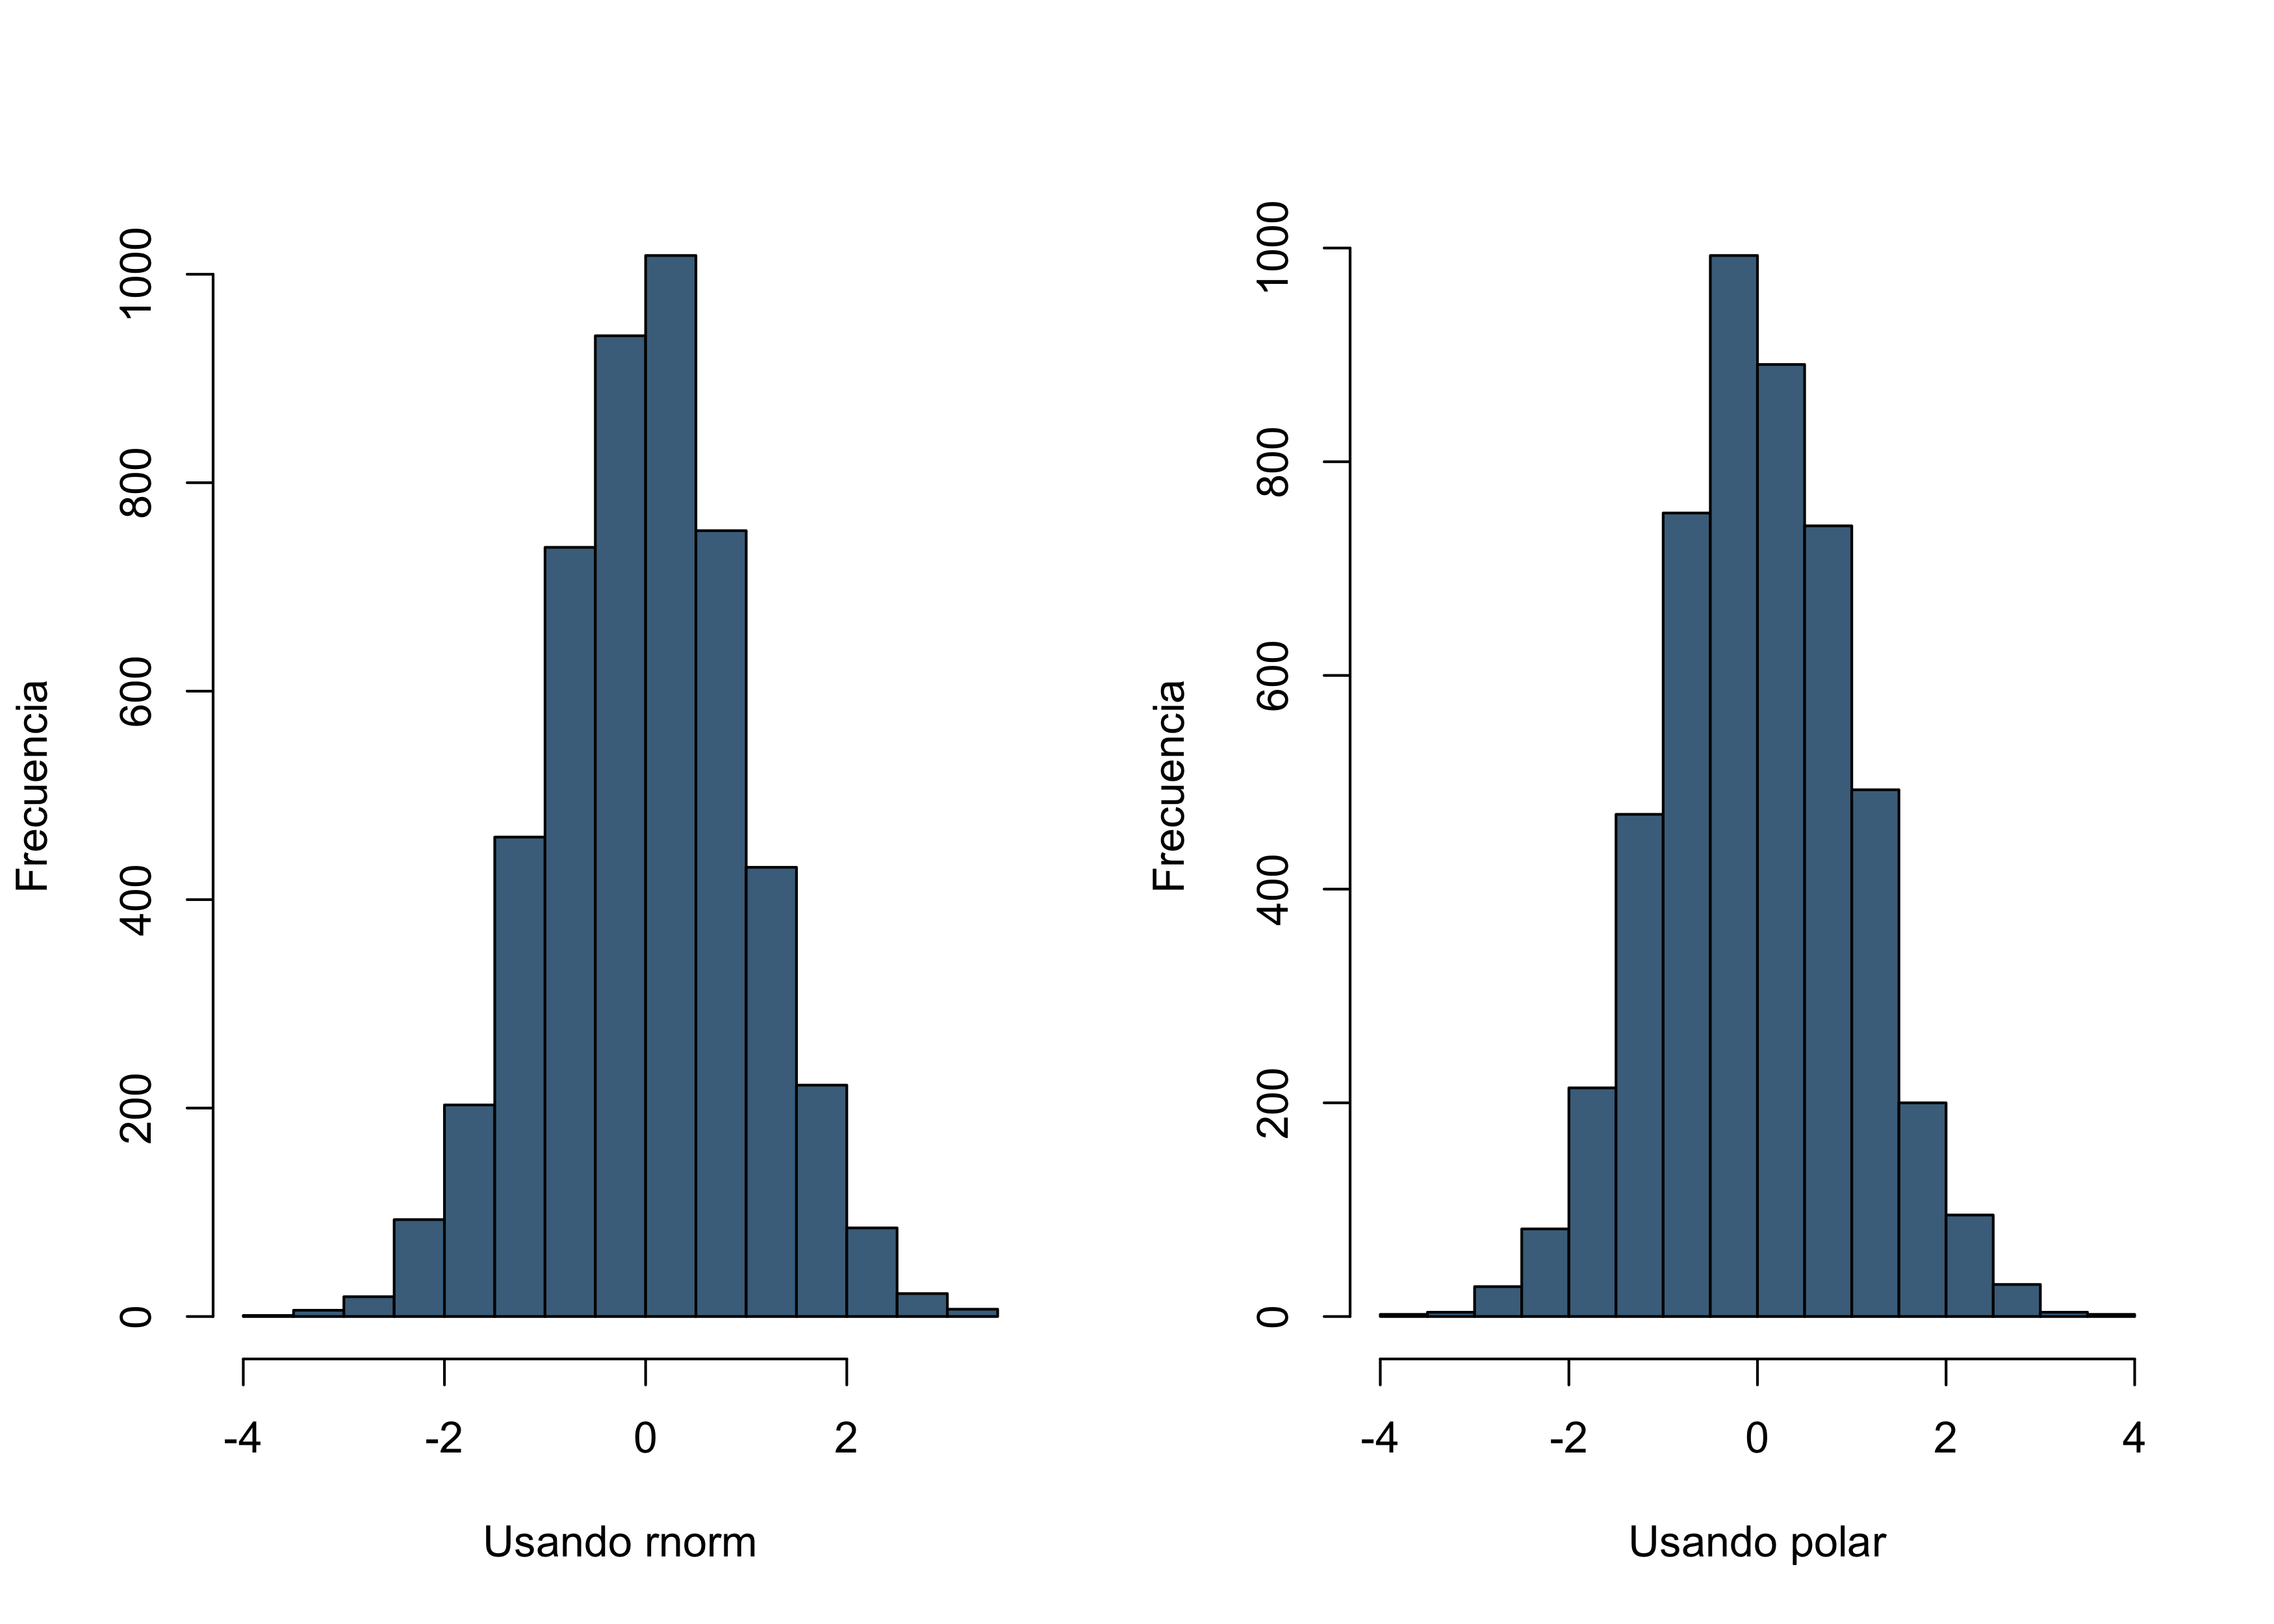
\includegraphics[scale=0.1]{polar.png}
\caption{Comparación de una réplica usando el \texttt{algoritmo polar} con \texttt{rnorm}.} 	
\label{polar}
\end{figure} 

Se realiza un experimento, realizando 500 réplicas donde en cada una se generan 5000 variables aleatorias y se les somete a una prueba de normalidad de Shapiro, de las cuáles 474 pasaron la prueba. 


\subsection{Teorema del límite central}
Este algoritmo se basa, en el \textit{teorema del límite central} \cite{int}. 
\begin{theorem}
Dadas variables aleatorias $T_1, T_2, \ldots, T_n$, independientes y con distribución cualquiera, se tiene que
$$\frac{\bar{T}-\mu_T}{\frac{\sigma_T}{\sqrt{n}}} = \frac{\sqrt{n}\left(\frac{1}{n}\sum^n_{i=1} (T_i - E(T_1\right))}{\sqrt{Var(T_1)}} \sim N(0,1)$$
si $n$ es suficientemente grande.
\end{theorem}

Usando una distribución que es fácil determinar, como la distribución uniforme, y $n=50$, tenemos el \textit{algoritmo basado en el TLC}.

\begin{algorithm}
  \caption{Algoritmo basado en el TLC}
  \begin{algorithmic}[1]
    \Ensure{$z_0$ variable con distribución normal}
 
    \State Generar  $u_1, u_2, \ldots, u_{50} \sim U(0,1)$ 
    \State Devolver $x=u_1+u_2+\ldots + u_{50} - 25$ 

 
  \end{algorithmic}
\end{algorithm}

\begin{figure}
\centering
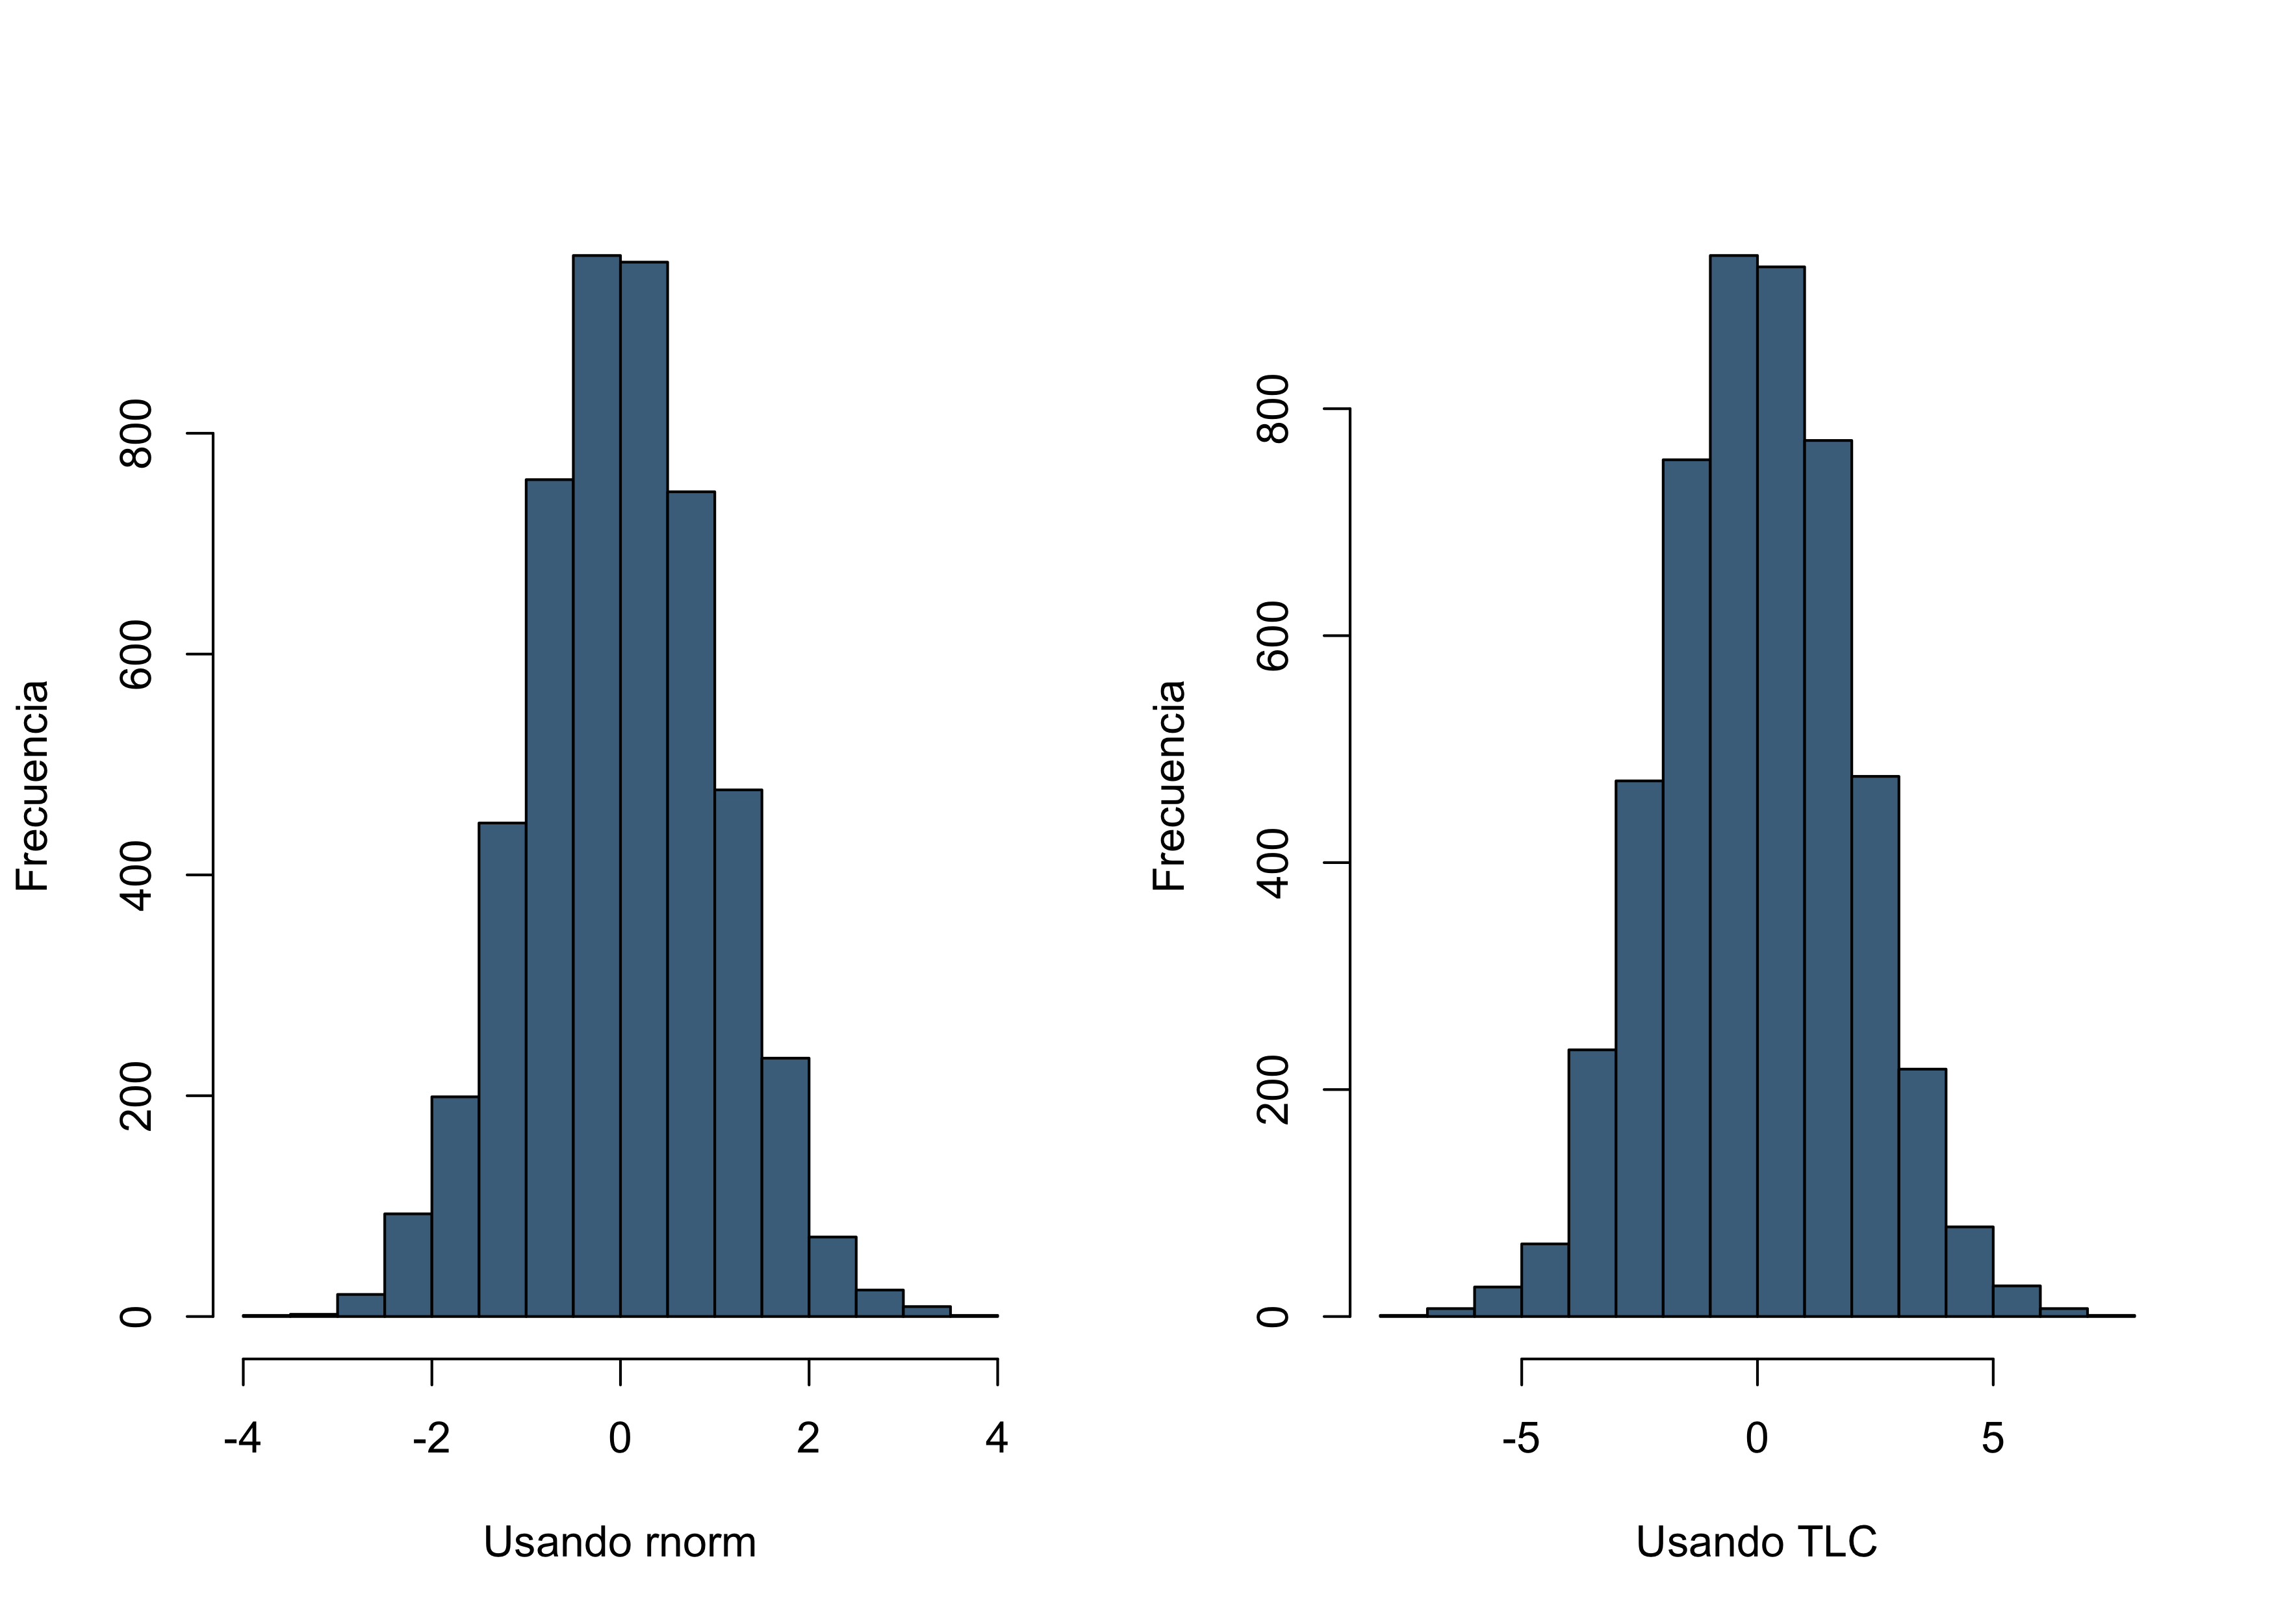
\includegraphics[scale=0.1]{tlc.png}
\caption{Comparación de una réplica usando el \texttt{algoritmo basado en TLC} con \texttt{rnorm}.} 	
\label{polar}
\end{figure} 

Se realiza un experimento, realizando 500 réplicas donde en cada una se generan 5000 variables aleatorias y se les somete a una prueba de normalidad de Shapiro, de las cuáles 482 pasaron la prueba. 

\section{Conclusiones}
En la figura \ref{boxplot} tenemos gráficos de caja que muestran los valores p resultantes de aplicar la prueba de Shapiro a muestras generadas por las tres variaciones del \textit{algoritmo Box-Muller}, el \textit{algoritmo polar} y \textit{el basado en el TLC}, en dicha figura, la línea roja está ubicada en el \texttt{valor p} = 0.05. Se aprecia que para los tres algoritmos, las muestras en su mayoría pasan las pruebas de normalidad normalidad.
\begin{figure}
\centering
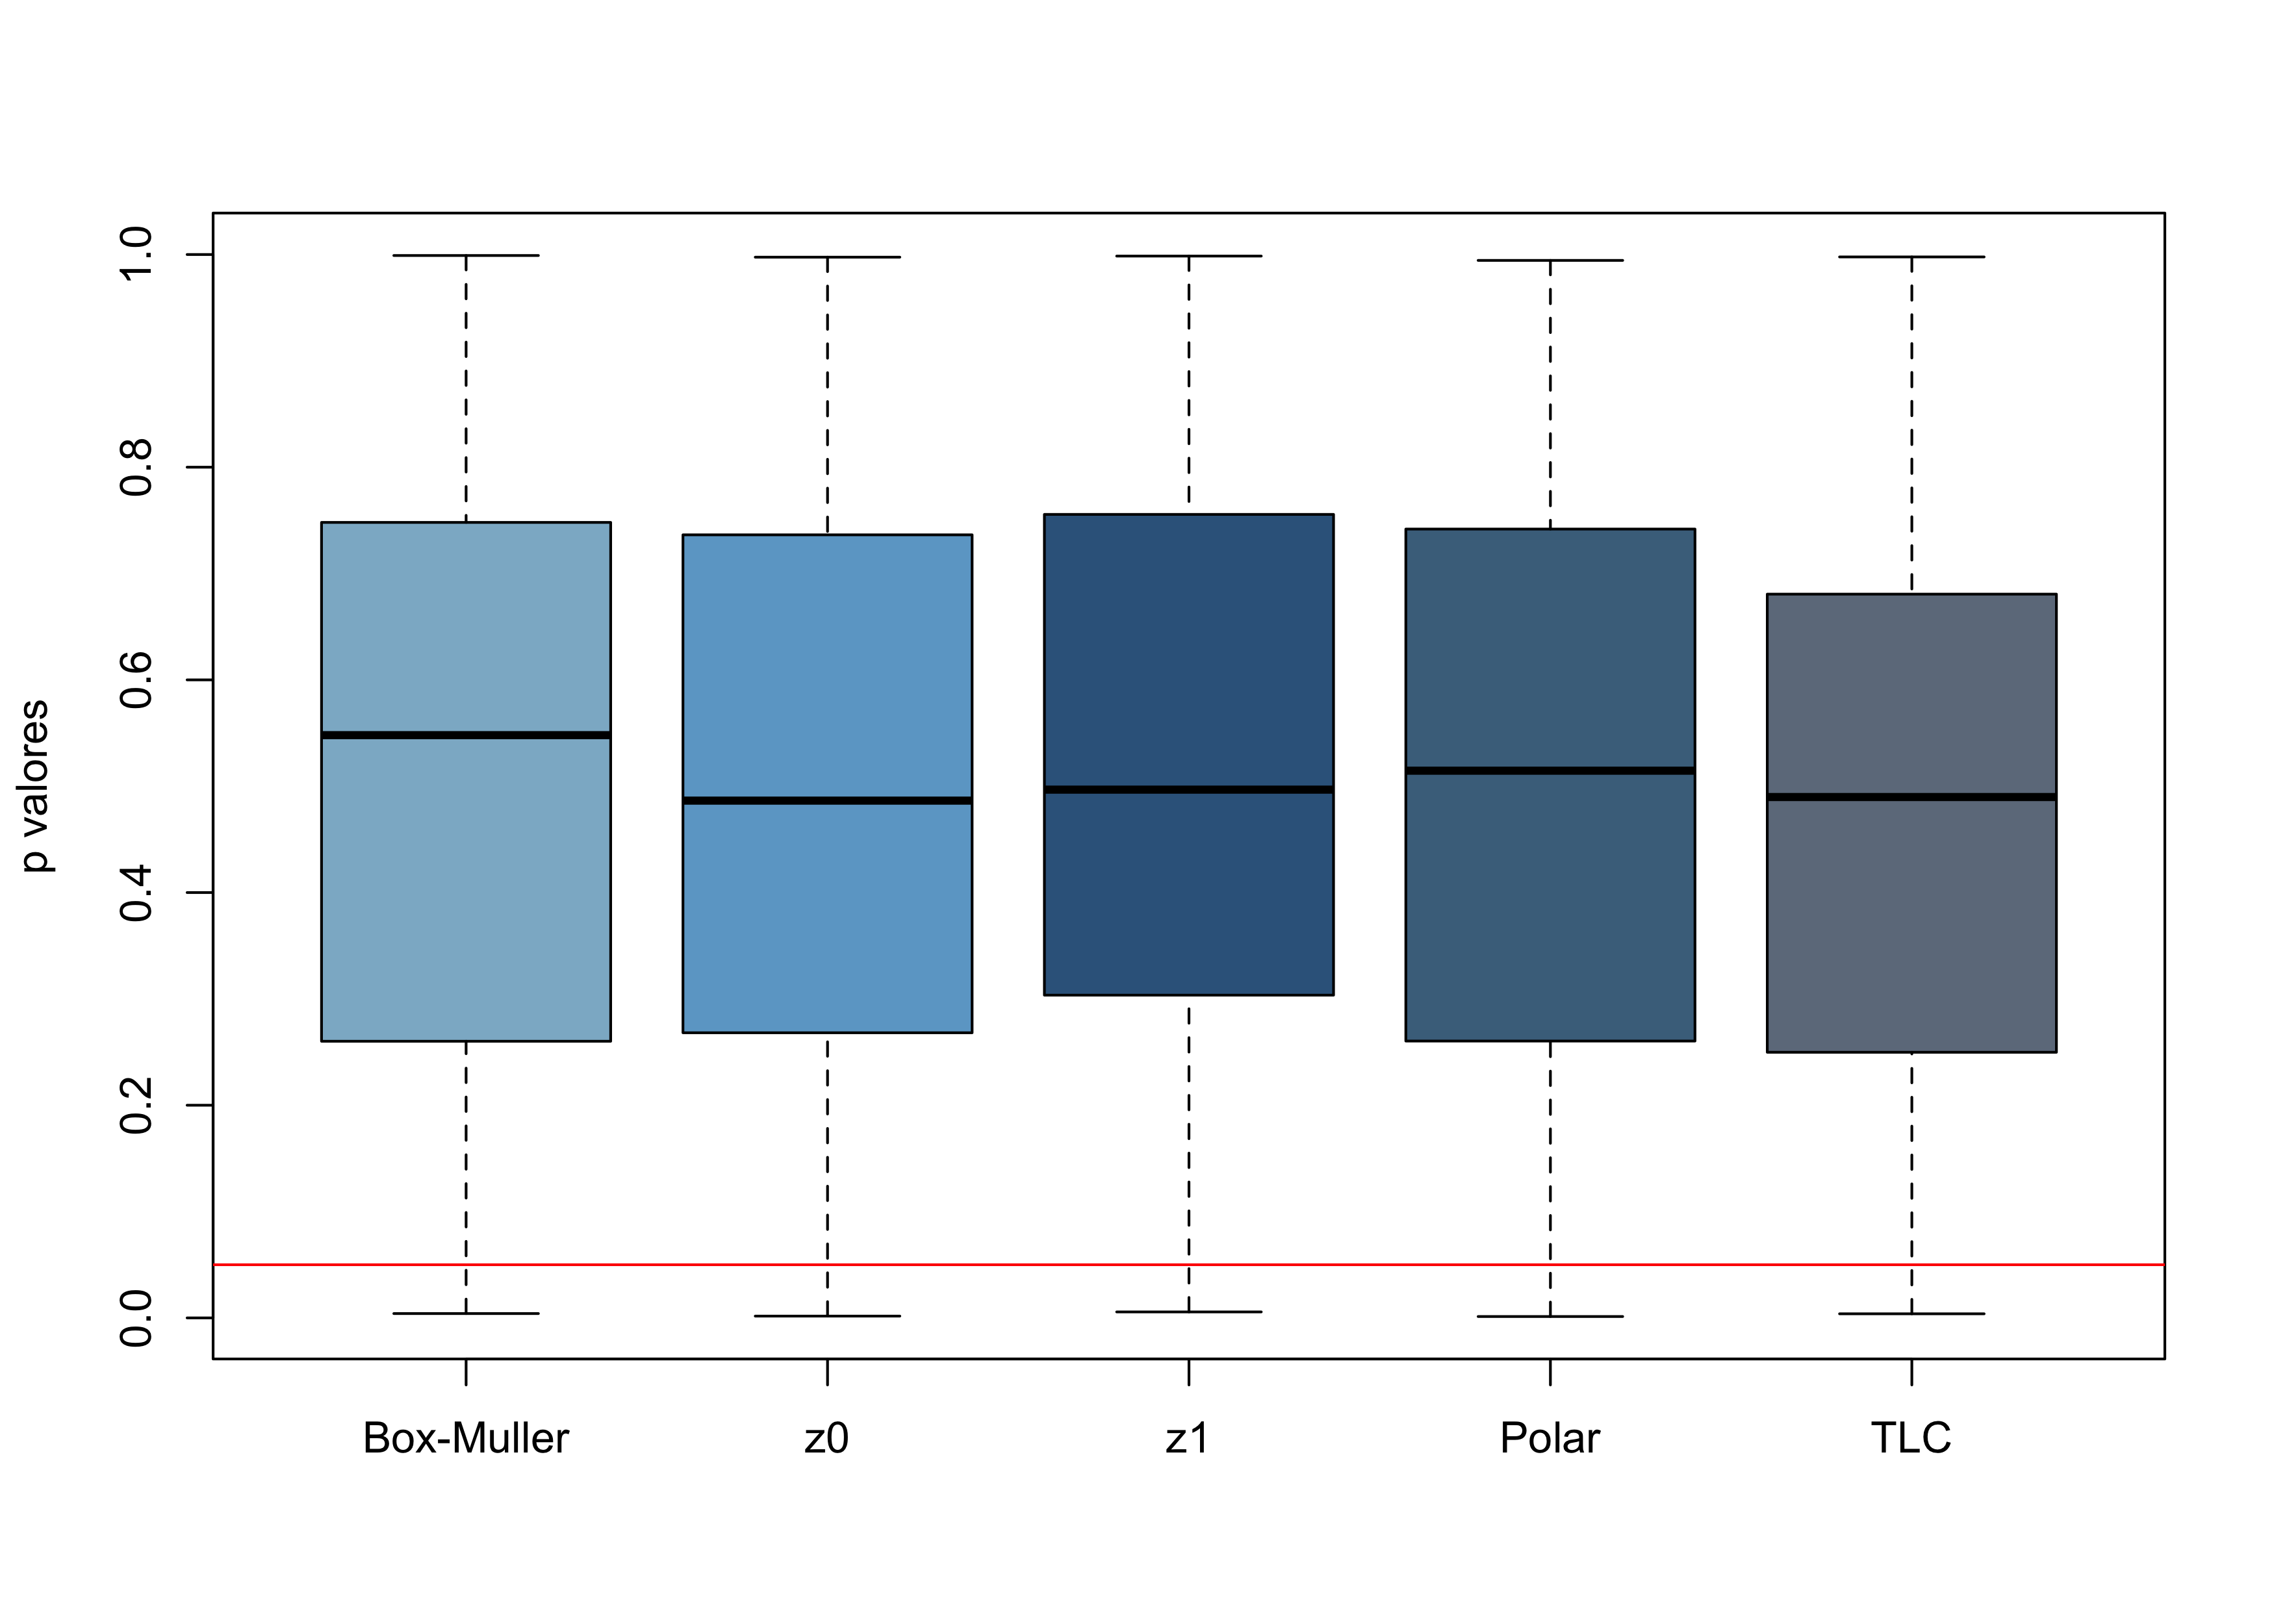
\includegraphics[scale=0.1]{boxplot.png}
\caption{Gráficos de caja con los valores p obtenidos en los experimentos.} 	
\label{boxplot}
\end{figure} 

\bibliographystyle{plain} 
\bibliography{Referencias}


\end{document} 